\documentclass[oribibl]{llncs}
 
\usepackage{amssymb} % AMS Fonts
\usepackage{amsmath} % AMSLaTeX
\usepackage{url}
\usepackage[pdftex]{graphicx}

% Compile only with pdfLaTeX
\usepackage[pdftex]{graphicx}

\newcommand{\ZZ}{{\mathbb{Z}}}
\newcommand{\QQ}{{\mathbb{Q}}}
\newcommand{\RR}{{\mathbb{R}}}
\newcommand{\CC}{{\mathbb{C}}}
\newcommand{\NN}{{\mathbb{N}}}
\renewcommand{\H}{{\mathcal{H}}}
\renewcommand{\L}{{\mathcal{L}}}
\newcommand{\F}{{\mathsf{F}}}
\newcommand{\bigO}{{\mathsf{O}}}
\newcommand{\R}{{\mathsf{R}}}
\newcommand{\Fp}{{\mathbb{F}_p}}
\newcommand{\Fq}{{\mathbb{F}_q}}
\newcommand{\Fqd}{{\mathbb{F}_{q^d}}}
\newcommand{\Fqe}{{\mathbb{F}_{q^e}}}
\newcommand{\Fz}{{\F[z]}}
\newcommand{\Fzf}{{\Fz /(f)}}
\newcommand{\Fzfe}{{\Fz /(f^e)}}
\newcommand{\Rn}{{\R^{n \times 1}}}
\newcommand{\Rnn}{{\R^{n \times n}}}
\newcommand{\Fden}{{\F^{den \times 1}}}
\newcommand{\Fdenden}{{\F^{den \times den}}}
\newcommand{\ZZp}{{\ZZ_p}}
\newcommand{\ZZpe}{{\ZZ_{p^e}}}
\newcommand{\nxn}{{n\times n}}
\newcommand{\calI}{{\mathcal I}}

\newcommand{\FD}{{\F[\partial;\sigma,\delta]}}
\newcommand{\D}{{\partial}}
\newcommand{\shift}{{\mathcal{S}}}
\newcommand{\diff}{{\lower3pt\hbox{\large$'$}}}
\renewcommand{\k}{{\mathsf{k}}}
\newcommand{\lclm}{{\mbox{\upshape lclm}}}
\newcommand{\lcrm}{{\mbox{\upshape lcrm}}}
\newcommand{\gcld}{{\mbox{\upshape gcld}}}
\newcommand{\gcrd}{{\mbox{\upshape GCRD}}}



\newcommand{\smallskipback}{\vspace{-\smallskipamount}}
\newcommand{\medskipback}{\vspace{-\medskipamount}}
\newcommand{\bigskipback}{\vspace{-\bigskipamount}}



%\reversemarginpar
\makeatletter
\@twosidefalse
\makeatother
%\renewcommand*{\marginfont}{\color{red}\bf}
%\newcommand{\TODO}[1]{\marginnote[#1]{}}

\textwidth180mm
\hoffset-30mm

\bibliographystyle{alpha}

\begin{document}

\title{ Skip Lists, Jump Lists, and Other Randomized Data Structures for Maintaining Ordered Sets}

\author{Bairong Lei, Michael Wexler}

\institute{University of Waterloo, David R. Cheriton School of Computer Science}

\maketitle

\begin{abstract}
  In this project, we will discuss several probabalistic data structures for maintaining ordered sets. These
  data structures use probabalistic methods to keep balanced, which helps to avoid skewed distributions that
  can lead to excessive running times. 
\end{abstract}

%%%%%%%%%%%%%%%%%%%%%%%%%%%%%%%%%%%%%%%%%%%%%%%%%%

\section{Introduction}

The need for ordered sets is very common in computer science. By ordered set, we mean a typical set data structure which has the additional property of maintaining the order of its elements. Programmers often need
such a structure in order to determine if a given element is in the set, and also to find the nearest predecessor for a given element. Given the functionality of an ordered set, it can be extended so that every 
key maps to a certain value. This would essentially be a dictionary data structure. One would hope that the most common dictionary operations would take O(log n), or better yet, O(1) time.

There has been much work in developing set data structures that provide O(log n) lookup time. Examples of these are hash-tables, AVL trees, and red-black trees. In addition to quick lookup times, AVL trees and red-black trees have the additional property of being able to provide O(log n) time for the next-predecessor operation, which, for a given key, will give the smallest key that is greater than that key.

For the afforementioned dictionary data structures, there is often the occurence where 

For instance, for a given n, if we were to insert the sequence 1 2 ... n into a normal binary search tree, we would end up having a very skewed structure, which would could take O(n) time to find an element. This is the reason AVL and red-black trees were developed. They use deterministic methods to perform self-balancing, so the skewed distribution never occurs.

The afforementioned data structures in their classical implementations all use deterministic methods for organizing their data.  Oftentimes, one wants to put a certain element of randomness into their dictionary data structures in order to avoid situations where their data structure becomes skewed. In this paper we will discuss various data structures that use randomness in order to maintain a level of balance, to avoid skewed distributions.

This paper is organized as follows: section \ref{sctn:randomized_data_structures} will give an overview on several probabalistic set data structures. Section \ref{sctn:experiments} will give an overview on some experiments we performed in order to compare these data structures.

The last section draws a conclusion of our work.

All test files and program code we describe in this report can be found in our \textsc{GitHub} repository \url{https://github.com/wexlermi/cs840project}.

%%%%%%%%%%%%%%%%%%%%%%%%%%%%%%%%%%%%%%%%%%%%%%%%%%

\section{Randomized data structures}
\label{sctn:randomized_data_structures}

\subsection{Treaps}
The first randomized data structure we will talk about is the treap. Treaps are at their foundation binary-search-trees, with a certain amount of randomness that allows them to remain balanced in the average case. Every element in a treap has the binary-search-tree property, such that all the nodes in its right subtree are greater than the root, and all the nodes in its left subtree are less than the root. However, every node in a treap contains a priority value, in which the priority of a treap node is always higher than that of its children. When we insert a new element into the treap, we randomly assign it a priority, which is a random integer from a sufficiently large range to ensure there are no collisions. Then we put the element in the treap, in the place it would go if it were considered only as a binary search tree. Once it is put in its proper place in the treap, a sequence of rotations are performed to restore the priority requirement, while still maintaining proper place to make sure its key is in the proper order.

\begin{figure}[here]
\center
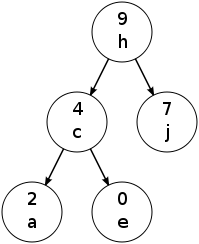
\includegraphics[width=7cm]{treap}
\caption{Example of a treap from http://en.wikipedia.org/wiki/File:TreapAlphaKey.svg}
\label{fig:treap}
\end{figure}

Figure \ref{fig:treap} is an example of a very small treap. The letters represent keys, and have the in-order property one would expect in a binary search tree. The numbers represent the priorities, in which case we have a max-heap, since each node has a priority greater than its children.

\subsection{Skip lists}
Skip lists are a randomized data structure that is inherently built upon ordinary linked-lists. Imagine we had a linked list of n numbers, in sorted order. If we had to search for an element x in this linked-list, it would be quite inefficient to linearly search for it. Instead, we can put pointers every other element, or every 3rd element, etc. This way, when searching for an element, we can first search through the top level, and once we find an element greater than it, we can drop down and search our original linked list.

We can repeat the process for the top linked list: put pointers to every other element. We keep repeating this process, where each higher level has half the pointers of the level below it, until we get a level which has 1 or 2 pointers. Then when we search for an element x, we start at the top list, skipping over elements that are less, then dropping down to lower and lower levels, repeating the process, until we either find the element we are looking for, or reach the bottom level and overshoot it, in which case we determine that the element does not exist in the skip list.

While the above description of a linked-list seems good at first, we reach a problem for insertion and deletion, in which case the length of the levels no longer have length $2^i$. Instead, we decide to use probabalistic methods to keep our levels approximately of length $2^i$. We specify a varible $p$ which represents the probability that an element on level $i$ will appear on level $i+1$. The typical value is $p=\frac{1}{2}$. Every time we would like to insert a key $x$ into the skip-list, we first put it at level 0. Then, we "flip a coin" a certain amount of times, and while we are getting heads, we keep adding the element to higher and higher levels, until we get a tails, and then we stop. This will mathematically ensure that our skip-list has approximately half the number of nodes at higher and higher levels, and provides us with good performance for insert and delete operations, something that is quite hard to maintain in deterministic skip-lists.

\begin{figure}[here]
\center
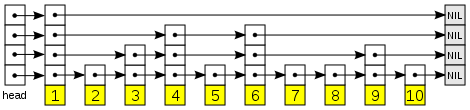
\includegraphics[width=7cm]{skip_list}
\caption{Example of a skip-list from \cite{skip_list}}
\label{fig:skip_list}
\end{figure}

\subsection{Skip lifts}

In \cite{skip_lift} Bose, Douïeb, Morin talk about an improvement to the skip list called the skip lift. A skip lift is a skip list in which every element only has the top two nodes. The rest are deleted. This greatly reduces the size of the skip list.

\section{Implementation}
\label{sctn:implementation}

For this project, we decided to implement the skip lift \cite{skip_lift}. We built our implementation off an implementation of the skip list \cite{skip_list_imp}. We also implemented the jump list\cite{jump_list}.  Our implementations can be found on our GitHub here: \url{http://github.com/wexlermi/cs840project}.

 \section{Experiment and Analysis}
\label{sctn:experiment}

We thought it would be interesting to collect metrics on runtime and datasize of these data structures, to see which ones perform most competitively from a time and space performance perspective. We conjectured that the skip lift would take less space than the skip list.


\begin{remark}
Hello
\end{remark}

\begin{itemize}
  \item The executable file that was compiled by \texttt{crestc}
  \item A number of maximal iterations through the control flow graph
    we want to allow (i.e. a limitation to the paths we
    want to consider. Otherwise the program might run too long)
  \item A strategy \textsc{CREST} should use to traverse the control
    flow graph. Possible options here are in the set
\begin{center}
$\{$\texttt{dfs}, \texttt{cfg}, \texttt{random},
    \texttt{uniform\_random}, \texttt{random\_input}, 
    \texttt{cfg\_baseline}, \texttt{hybrid}$\}$
\end{center}
\end{itemize}


\begin{table}[htbp]
\caption{DFS branch-coverage-ratio}
\begin{center}
\begin{tabular}{|r|r|r|r|r|r|}
\hline
1 & 1 & 1 & 1 & 1 & 1 \\ \hline
2 & 0.75 & 0.75 & 0.25 & 0.25 & 0 \\ \hline
3 & 0.667 & 0.667 & 0.667 & 0.333 & 0 \\ \hline
4 & 0.625 & 0.75 & 0.25 & 0 & 0 \\ \hline
5 & 0.6 & 0.7 & 0.6 & 0 & 0 \\ \hline
\end{tabular}
\end{center}
\label{DFS timings (in seconds)}
\end{table}


\begin{figure}[!t]
\centering
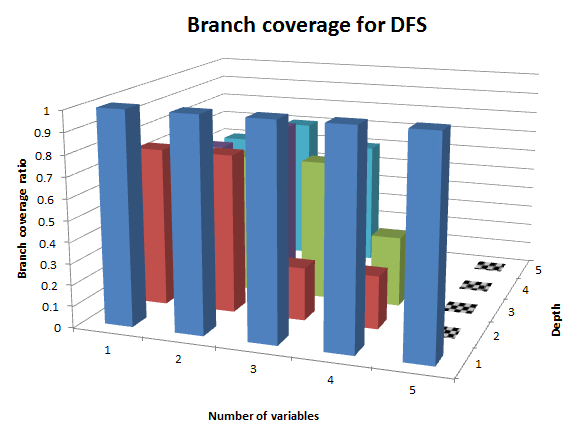
\includegraphics[width=9cm]{dfs_branch_coverage}
\caption{}
\label{figure:motivation}
\end{figure}
%%%%%%%%%%%%%%%%%%%%%%%%%%%%%%%%%%%%%%%%%%%%%%%%%%

\section{Conclusion and Future Work}
\label{sctn:Conclusion}

There are several conclusions we can draw in this report.


\bibliographystyle{plain}
\bibliography{report1}

\end{document}
